% Options for packages loaded elsewhere
\PassOptionsToPackage{unicode}{hyperref}
\PassOptionsToPackage{hyphens}{url}
%
\documentclass[
]{article}
\usepackage{amsmath,amssymb}
\usepackage{iftex}
\ifPDFTeX
  \usepackage[T1]{fontenc}
  \usepackage[utf8]{inputenc}
  \usepackage{textcomp} % provide euro and other symbols
\else % if luatex or xetex
  \usepackage{unicode-math} % this also loads fontspec
  \defaultfontfeatures{Scale=MatchLowercase}
  \defaultfontfeatures[\rmfamily]{Ligatures=TeX,Scale=1}
\fi
\usepackage{lmodern}
\ifPDFTeX\else
  % xetex/luatex font selection
\fi
% Use upquote if available, for straight quotes in verbatim environments
\IfFileExists{upquote.sty}{\usepackage{upquote}}{}
\IfFileExists{microtype.sty}{% use microtype if available
  \usepackage[]{microtype}
  \UseMicrotypeSet[protrusion]{basicmath} % disable protrusion for tt fonts
}{}
\makeatletter
\@ifundefined{KOMAClassName}{% if non-KOMA class
  \IfFileExists{parskip.sty}{%
    \usepackage{parskip}
  }{% else
    \setlength{\parindent}{0pt}
    \setlength{\parskip}{6pt plus 2pt minus 1pt}}
}{% if KOMA class
  \KOMAoptions{parskip=half}}
\makeatother
\usepackage{xcolor}
\usepackage[margin=1in]{geometry}
\usepackage{graphicx}
\makeatletter
\def\maxwidth{\ifdim\Gin@nat@width>\linewidth\linewidth\else\Gin@nat@width\fi}
\def\maxheight{\ifdim\Gin@nat@height>\textheight\textheight\else\Gin@nat@height\fi}
\makeatother
% Scale images if necessary, so that they will not overflow the page
% margins by default, and it is still possible to overwrite the defaults
% using explicit options in \includegraphics[width, height, ...]{}
\setkeys{Gin}{width=\maxwidth,height=\maxheight,keepaspectratio}
% Set default figure placement to htbp
\makeatletter
\def\fps@figure{htbp}
\makeatother
\setlength{\emergencystretch}{3em} % prevent overfull lines
\providecommand{\tightlist}{%
  \setlength{\itemsep}{0pt}\setlength{\parskip}{0pt}}
\setcounter{secnumdepth}{-\maxdimen} % remove section numbering
\ifLuaTeX
  \usepackage{selnolig}  % disable illegal ligatures
\fi
\IfFileExists{bookmark.sty}{\usepackage{bookmark}}{\usepackage{hyperref}}
\IfFileExists{xurl.sty}{\usepackage{xurl}}{} % add URL line breaks if available
\urlstyle{same}
\hypersetup{
  pdftitle={Waveforms},
  pdfauthor={Diego},
  hidelinks,
  pdfcreator={LaTeX via pandoc}}

\title{Waveforms}
\author{Diego}
\date{2023-05-19}

\begin{document}
\maketitle

\hypertarget{modulaciuxf3n-de-ancho-de-pulso-pwm}{%
\section{Modulación de Ancho de Pulso
(PWM)}\label{modulaciuxf3n-de-ancho-de-pulso-pwm}}

\hypertarget{pwm}{%
\subsubsection{PWM}\label{pwm}}

La señal PWM (Pulse Width Modulation, Modulación de Ancho de Pulso) es
una señal que utiliza el microcontrolador para generar una señal
continua sobre el proceso a controlar.

\hypertarget{ciclo-de-trabajo}{%
\subsubsection{Ciclo de trabajo}\label{ciclo-de-trabajo}}

El ciclo de trabajo, a veces denominado ``factor de trabajo'', se
expresa como un porcentaje del tiempo de activación. Por ejemplo, un
ciclo de trabajo del 10\% es una señal que se encuentra activada el 10\%
del tiempo y desactivada el otro 90\%.

\begin{figure}
\centering
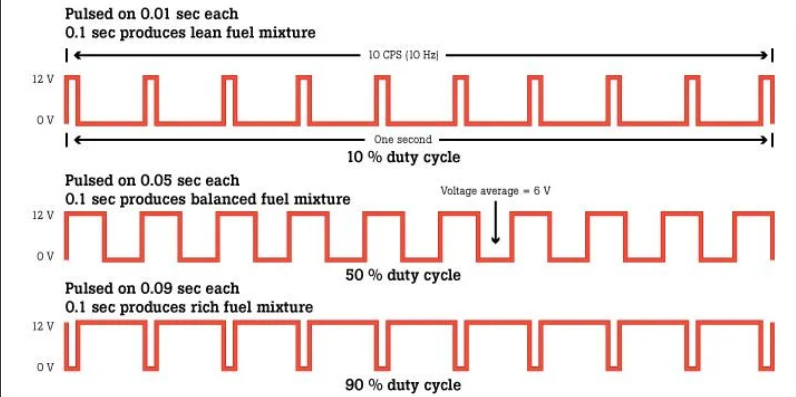
\includegraphics{images/Duty.png}
\caption{DutyCycle}
\end{figure}

\hypertarget{simulacion-en-multisim}{%
\subsubsection{Simulacion en Multisim}\label{simulacion-en-multisim}}

\begin{verbatim}
Señales cuadradas solicitadas:
\end{verbatim}

\begin{figure}
\centering
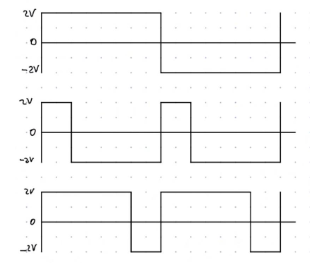
\includegraphics{images/SQ2.png}
\caption{Señales Cuadradas}
\end{figure}

Para simular las señales cuadradas solicitadas deben seguirse los
siguientes pasos:

\begin{enumerate}
\def\labelenumi{\arabic{enumi}.}
\tightlist
\item
  Seleccionar el modo de onda cuadrada en el generador de funciones
  Agilent
\end{enumerate}

\begin{figure}
\centering
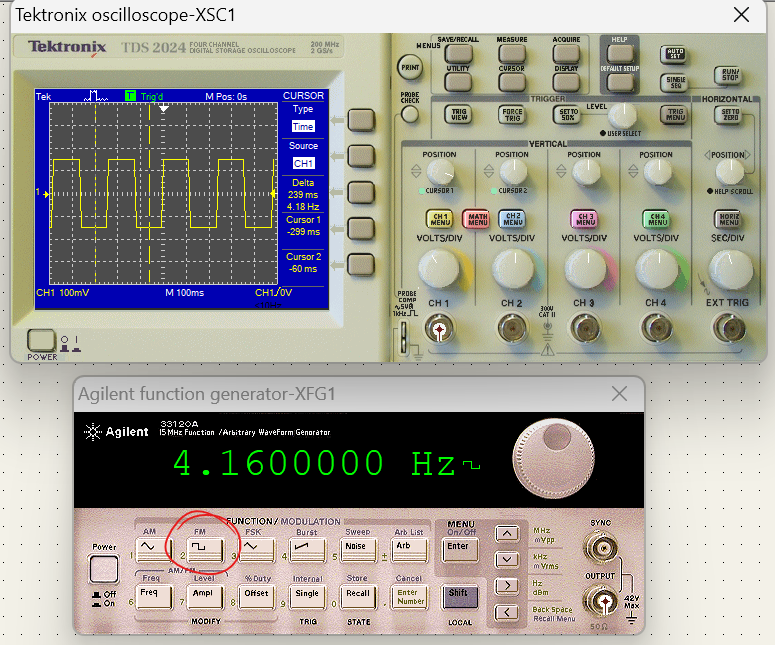
\includegraphics{images/CD1.png}
\caption{SQ}
\end{figure}

\begin{enumerate}
\def\labelenumi{\arabic{enumi}.}
\tightlist
\item
  Especificar la frecuencia a partir de la expresión
\end{enumerate}

\[\omega = 5\pi \frac{kRads}{s}\]

Siendo \(\omega\) la frecuencia angular en kilo radianes y conociendo
que

\[\omega = \frac{2 \pi}{T} \ \ y \ \ f = \frac{1}{T}\]

por tanto

\[5\pi = \frac{2\pi}{T}\]

\[\frac{5\pi}{2\pi} = \frac{1}{T}\]

\[\frac{5\cancel{\pi}}{2\cancel{\pi}} = f\]

\[\boxed{Frecuencia \rarr 2.5kHz = f}\]

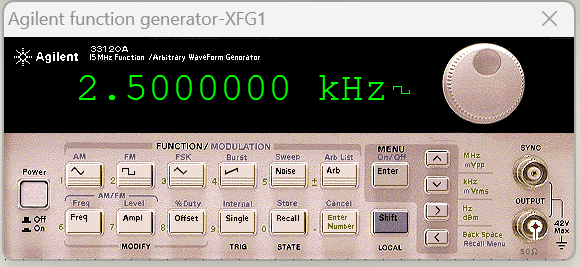
\includegraphics{2023-05-18-20-29-16.png}

\begin{enumerate}
\def\labelenumi{\arabic{enumi}.}
\setcounter{enumi}{1}
\tightlist
\item
  Calcular el periodo de la señal
\end{enumerate}

\[f = 2.5kHz = 2500Hz\]

\[T = \frac{1}{f}\]

\[T = \frac{1}{2500Hz}\]

\[\boxed{Periodo \rarr T = 0.0004s = 400\mu s} \]

\begin{enumerate}
\def\labelenumi{\arabic{enumi}.}
\setcounter{enumi}{2}
\tightlist
\item
  Establecer el \(V_{pp}\) en el generador
\end{enumerate}

A partir de las figuras proporcionadas de las señales solicitadas,
podemos identificar que la amplitud es de 2V o, lo que es lo mismo, un
voltaje pico a pico de \(V_{pp} = 4V\).

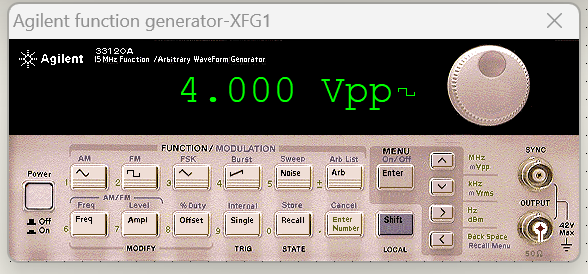
\includegraphics{2023-05-18-20-47-36.png}

\begin{enumerate}
\def\labelenumi{\arabic{enumi}.}
\setcounter{enumi}{3}
\tightlist
\item
  Ajustar las escalas de voltaje y tiempo en el osciloscopio
\end{enumerate}

En este caso se emplearon divisiones de 2V para la escala del voltaje y,
a su vez, se emplearon divisiones de 100\(\mu\)s para la escala del
tiempo.

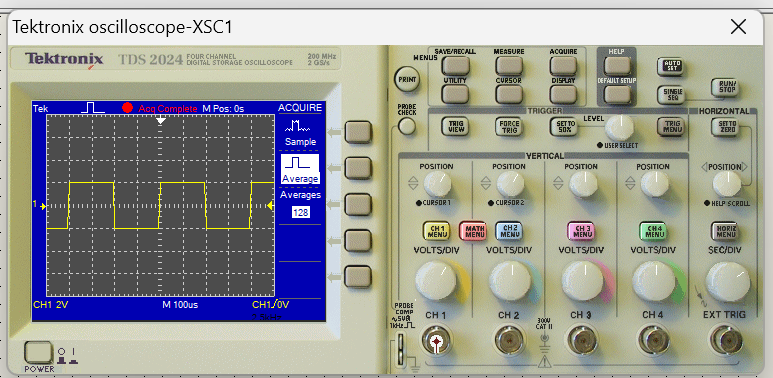
\includegraphics{2023-05-18-20-59-38.png}

\begin{enumerate}
\def\labelenumi{\arabic{enumi}.}
\setcounter{enumi}{4}
\tightlist
\item
  Ajustar el ciclo de trabajo
\end{enumerate}

Para ajustar el ciclo de trabajo se debe presionar el botón
\texttt{Shift} del generador de funciones y posteriormente el botón
\texttt{Offset} , mismo que cuenta con leyenda de \texttt{\%\ Duty}.

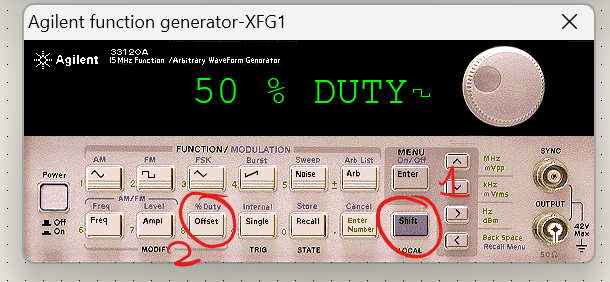
\includegraphics{2023-05-18-21-06-09.png}

\end{document}
